% Explain the implementation of the library rust-debug

% Explain why this library was made.
Retrieving debug information from the \gls{DWARF} sections in the \gls{elf} file is one of the main problems that needs to be solved when creating a debugger.
The \emph{Rust} library \emph{gimli-rs} simplifies that problem by providing data structures and functions for reading the \gls{DWARF} sections.
However, the library requires a lot of knowledge about the \gls{DWARF} format to use.
Thus the \emph{rust-debug} library was created to make it even easier to get the debug information.
Figure \ref{fig:rustdebug} shows how the two libraries and the \gls{elf} file are connected.


\begin{figure}[h]
	\centering
	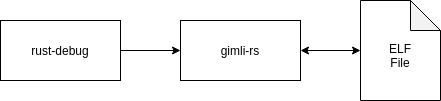
\includegraphics[width=1.0\textwidth]{rust_debug.png}
	\caption{A diagram showing the relation between the \emph{ELF} file and the two libraries \emph{rust-debug} and \emph{gimli-rs}.}
	\label{fig:rustdebug}
\end{figure}


Some of the main functionality that \emph{rust-debug} provides are the following:

\begin{itemize}
  \item Retrieving the source file location for functions, variables, types and more.
  \item Virtually unwinding the call stack.
  \item Evaluating variables.
  \item Translating source file line number to the nearest machine code address.
  \item Finding the \gls{die} that represents a function using the name.
\end{itemize}

There is more functionalities that \emph{rust-debug} provides but they are not noteworthy.
The code of this library is in the \emph{GIT} repository \cite{rust-debug}.



\subsubsection{Retrieving Source File Location}
% Explain the evaluation of source informaiton % TODO
Some of the \glspl{die} in \gls{DWARF} have attributes that starts with \emph{DW\_AT\_decl\_}.
These attributes contain information on where in the source file the \gls{die} was declared.
This include file path, line number and column number.
The library \emph{rust-debug} has a function for retrieving the value of all these attributes from a given \gls{die}.


The attribute  \emph{DW\_AT\_decl\_file} which contain the file path of where the \gls{die} was declared has a file index as its value.
Every compilation unit has a line number information table that contain file paths which are indexed.
Thus the \emph{rust-debug} library will search for the matching index in the table to find the file path.
Finding the line and column number does not require any lookup.


\subsubsection{Accessing Memory And Registers}
% Explain the evaluation part. % TODO
% Explain the stored target memory and registers
One of the requirements for evaluating the value of a variable is access to the registers and memory of the debug target.
\emph{rust-debug} does not have that functionality because it should be hardware independent as much as possible.
Instead, the library uses a data structure which contain the values of the registers and memory.
This keeps the library hardware independent.
The data structure also has some function for reading and adding values.
Thus it is the user of the library that has to add the values to the data structure.


The register and memory data structure is used as an argument to the functions in the library.
If a value is missing, the called function will return a result that describes which value is missing.
Then the user of the library can read that value from the debug target, and add it to the data structure.
If there are more values missing then calling the function with the updated values will signal that additional values needs to be added.
This repeats until the function give a result that says it has completed its task.


\subsubsection{Evaluating Variables} \label{sec:ievalvar}
% Explain the evaluation of vairbles.
The \emph{rust-debug} library has a structure called \emph{VariableCreator}, it takes a reference to a \gls{DWARF} unit and \gls{die}.
The \gls{die} has to be one that represents a variable.
When the data structure is created, it will extract some important information about the variable from the \gls{die}. A constructed \emph{VariableCreator} struct has a method for evaluating the value of the variable that requires the register and memory data structure.
This method evaluates the variable as described in section \ref{sec:evaluate-variable} and the \gls{DWARF} specification \cite{dwarf}.
The return value of the method is an enum that is used for telling the user if a value is missing from the register and memory data structure or not.
Then there exists another method for retrieving the variable information containing the evaluated value.
The variable information contains the following:

\begin{itemize}
  \item Variable name.
  \item Variable type.
  \item Variable location in the source file.
  \item The locations of the variable value in registers and memory.
  \item The evaluated value of the variable.
\end{itemize}


\subsubsection{Finding a functions DIE} \label{sec:funcdie}
The \emph{rust-debug} library has a function for finding a \gls{die} that represents a function using the name of that function.
The function also needs a machine code address to find the correct compilation unit.


The correct compilation unit can be found using a code address.
Every compilation unit has an address range that can be used to see if the machine code is from that compilation unit.
Thus searching for the correct one is done by going through each unit, and checking if the address is in the range.


When the compilation unit is known, the \gls{die} representing the subroutine can be found by searching the \gls{die} tree of the unit.
This is done by going down the path of the tree where the machine code address is in range.
It returns a result when it has found the subroutine \gls{die} with the searched name, or when there are no more \glspl{die} to check.


\subsubsection{Unwinding Call Stack}
% Explain the evaluation of call stack % TODO
% Explain the evaluation of stackframe 
The \emph{rust-debug} library has a data structure called \emph{Stacktrace}, which works very similarly to the data structure describe in section \ref{sec:ievalvar}.
However, \emph{Stacktrace} is used to virtually unwind the call stack and evaluate all the variables in it.
The call stack is unwound as described in section \ref{sec:stacktrace} and the \gls{DWARF} specification \cite{dwarf}.
This results in a stack of activations, which most importantly contain restored register values and stack pointers.


All the variables in each of the activations are then evaluated using the restored register values.
This is done using a data structure that works similar to the data structure describe in section \ref{sec:ievalvar}.

The first step of evaluating the variables is finding the \gls{die} of the subroutine that the activation is related to.
This is done using the function described in section \ref{sec:funcdie}.
After that the \gls{die} tree is searched through for variable \glspl{die}, starting at the subroutine \gls{die}.
All the variable \glspl{die} found are added to a list.
Each variable in the list is then evaluated as described in section \ref{sec:ievalvar}.
If there is a missing value from memory then the response from the evaluation of the variable is returned.
Because the data structure works similar to the one in section \ref{sec:ievalvar}, it can continue from were it last stopped.


\subsubsection{Finding Breakpoint Location}
% Explain how to get breakpoint locaiton.
The \emph{rust-debug} library has a function that finds a machine code location using a source file location.
This machine code location is the closest one that represents the line in the source code.
The function requires a file path and line number, but it also can take a column number.


The mentioned function works by first finding out which compilation unit contains information on the inputted file path.
It does this by looping through all the file entries in the line number information table for every compilation unit.
Each line number information table entry have rows that each contain information on a line from the source code.
Thus all the rows with the search line numbers are added to a list.
The machine code address of the first element in this list is returned if no column line was inputted to the function.
Otherwise, it is the one with the closest column number that is returned.

